\documentclass[oneside]{book}
\usepackage[T1]{fontenc}
\usepackage[utf8]{inputenc}
\usepackage{geometry}   
\usepackage{float}
\usepackage[section]{placeins}
\usepackage{amsmath}
\usepackage{amssymb}
\usepackage{amsfonts}
\usepackage[colorlinks=true, allcolors=blue]{hyperref}
\usepackage{mathtools}
\usepackage[switch, mathlines]{lineno}
\usepackage[usenames,dvipsnames]{xcolor} 
\usepackage[normalem]{ulem}
\usepackage[capitalise,nameinlink]{cleveref}
\usepackage{enumitem}
\usepackage{csquotes}
\usepackage{xspace}
\usepackage{multirow}
\usepackage{tabularx}
\usepackage{color, colortbl}
\usepackage[colorinlistoftodos]{todonotes}
\usepackage{graphicx}
\usepackage{caption}
\usepackage{subcaption}
% for writing code blocks 
\usepackage{listings}
%\usepackage{color}

\definecolor{orange}{rgb}{1,0.5,0}
\definecolor{darkorange}{rgb}{0.69,0.33,0.13}
\definecolor{fidcol}{rgb}{0.7,0,0}
\definecolor{mkcol}{rgb}{0.5,0,0.5}
\definecolor{mmcol}{rgb}{0.7,0.17,0.31}
\definecolor{dscol}{rgb}{0.6,0.1,0.2}
\definecolor{mccol}{rgb}{0.2,0.4,0.6}
\definecolor{darkgreen}{rgb}{0.05,0.5,0.06}
\definecolor{carnelian}{rgb}{0.7, 0.11, 0.11}
\definecolor{dkgreen}{rgb}{0,0.6,0}
\definecolor{mauve}{rgb}{0.58,0,0.82}
%table colors
\definecolor{gray}{gray}{0.9}
\definecolor{cyan}{rgb}{0.88,1,1}

\newcommand*{\Euclid}{\textit{Euclid}\xspace}
\newcommand*{\Planck}{\textit{Planck}\xspace}
\newcommand*{\rd}{\mathrm{d}}
\newcommand*{\rD}{\mathrm{D}}
\newcommand*{\marktodo}{{\color{mmcol} ::TODO::}\xspace}
\newcommand*{\halofit}{\texttt{HALOFIT}\xspace}
\newcommand*{\hmcode}{\texttt{HMCODE}\xspace}
\newcommand*{\montepython}{\texttt MP\xspace}
\newcommand*{\cosmicfish}{\texttt CF\xspace}
\newcommand*{\class}{\texttt CLASS\xspace}
\newcommand*{\camb}{\texttt CAMB\xspace}
\begin{document}
\chapter{Neutrinos and the Large Scale Structure}
In this chapter we will briefly discuss the effects that neutrinos have on the mater power spectrum. For a more in-depth discussion of all the effects that neutrinos have on our universe we reffere to the main source of this chapter \marktodo. In the first section we will give a phenomenological overview on the effect of massive neutrinos on the large scale structure. Then we will remark on the effect that additional massless neutrinos have on the matter power spectrum. These discussions will also be representative of other simple light dark matter models. Blandly said any relativistic, collisionless, thermalized particle acts like a neutrino on the large scale structure on the universe.
\section{Massive Neutrinos}  
When discussing the effect of the massive neutrinos on the power spectrum the main effect can be very roughly described with three main phenomenological statements:\begin{itemize}
    \item Massive neutrinos stop clustering on scales larger than their free streaming scale that is related to their velocity.
    \item Massive neutrinos lead to an overall steplike suppression of the power spectrum by an amount proportional to their mass.
    \item Massive neutrinos change the redshift of matter-to-radiation equality essentially shifting the peak of the matter power spectrum.
\end{itemize}
The first effect leads to a suppression of the power spectrum for scales smaller than some scale $k_*$. This can be understood from folowing reasoning. The free-streaming scale repesents a scale under which collisionless particles can not be confinded, if we define it analogously to the Jeans wavenumber we find a free-streaming wavenumber 
\begin{equation}
    k_\mathrm{fs} = \sqrt{\frac{3}{2}}\,\frac{a\,H}{c_\nu}
\end{equation}
For relativistic neutrinos $c_\nu$ is just one while for nonrelativistic neutrinos we can find the thermal verlocity by dividing the mean momentum by the neutrino mass. This leads to \begin{align}
    c_\nu =  &\approx \frac{8.78\cdot10^{-3}}{a}\,\frac{0.06\,\mathrm{eV}}{m_\nu} \nonumber \\
    k_\mathrm{fs} &\approx 4.66\cdot10^{-3}\,\frac{m_\nu}{0.06\,\mathrm{eV}}\,a^2\,\frac{H}{H_0}\,h\,\mathrm{Mpc}^{-1}.
\end{align}
During matter domination for the relativistic case the free streaming wavenumber falls with $\eta^{-1}$ and for the nonrelativistic case the wavenumber growths with $\eta$. This means that at the transition from relativistic to nonrelativistic we find the largest scale for at wich neutrinos stoped clustering. We denote this scale with $k_\mathrm{min}$ (we will call it the minimum clustering scale), and it is precisely where the steplike suppression of the neutrinos starts. Given that the transition to the nonrelativitic regime happens during matter domination, $k_\mathrm{min}$ can be approximated by 
\begin{equation}
    k_\mathrm{min} \approx 7.96\cdot10^{-3}\,\sqrt{\frac{\Omega_m}{0.3}}\,\sqrt{\frac{m_\nu}{0.06\,\mathrm{eV}}}\,h\,\mathrm{Mpc}^{-1}.
\end{equation}
To describe the second effect we first need to disect our matter perturbation into baryons, CDM and massive neutrinos. We can write 
\begin{equation}
    \label{eq:decomposition}
    \delta_m = f_c \,\delta_c + f_b\, \delta_b + f_\nu\,\delta_\nu.
\end{equation}
The factors $f_X$ are the fractoral contribution of the species $X$ to the toal energy density of the universe. The equations of moton drive the neutrino perturbations to an equilibrium similar to the cold constiuants. However, due to the high verlocity of the neutrinos, there is non-negligible pressure and anisotropic stress. 
This leads to \begin{itemize}
    \item[(a)] a small scale suppression of the neutrino perturbation that is approximately given by 
    \begin{align*}
        \delta_\nu \propto \left(\frac{k_\mathrm{fs}}{k}\right)^2\,\delta_c
    \end{align*} 
    on scales smaller than the freestreming scale.
    \item[(b)] a scale dependent growthrate that is reduced compared the cold matter constiuants until the equilibrium has been reached.
\end{itemize}
For the following discussion we will only look at what will happen to the matter perturbations for scales much larger than the minimum clustering scale. Because of the two reasons stated above, on these scales we use that at late times typical $|\delta_\nu|\ll\delta_c$. We can now expand equation \ref{eq:decomposition} to find \begin{align}
 &&\langle \delta_m(k)\,\delta^*_m(k')\rangle &\approx (f_c+f_b)^2\left\langle\frac{(f_c \,\delta_c(k) + f_b\, \delta_b(k))(f_c \,\delta_c^*(k') + f_b\, \delta_b^*(k'))}{(f_c + f_b)^2}\right\rangle \nonumber\\
&&&\coloneqq (f_c+f_b)^2 \langle \delta_{cb}(k)\,\delta_{cb}^*(k') \rangle \\
\Longleftrightarrow && P_{mm}(k) &\approx (1-f_\nu)^2 P_{cb}(k),
\end{align}
where we have defined the perturbation of the CDM+baryon field $\delta_{cb}$ and it's respective power spectrum. After the baryon drag epoch, i.e. after baryons decouble from the radiation field, the equations of motion for this new density contrast simplifies to 
\begin{equation}
    \delta_{cb}'' + \frac{a'}{a}\,\delta'_{cb} - 4\,a^2\,\pi\,G\,\langle \rho_c + \rho_b \rangle\, \delta_{cb} = 0,
\end{equation} 
where the prime denotes derivatives with respect to conformal time.\\
The third term is starting to look like the Friedmann–Lemaître equation minus the effect of massive neutrinos. If we add them we can write 
\begin{equation}
    \delta_{cb}'' + \frac{a'}{a}\,\delta'_{cb} - \frac{3}{2}\,(1-f_\nu)\left({a'}\right)^2 \delta_{cb} = 0.
\end{equation}
Lets assume that we are deep into matter domination such that the bulk of neutrinos are allready non-relativistic. The neutrino density thus scales with $a^{-3}$. At this time the background evolution matches the neutrinoless case, and we can write that $a\propto\eta^2$. If we instert the conformal time into the equality we can solve the differential equation to find \begin{align}
    &\delta_{cb}'' + \frac{2}{\eta}\,\delta'_{cb} - \frac{6}{\eta^2}\,(1-f_\nu) \delta_{cb} = 0.\\
    \Longrightarrow\quad&\delta_{cb} \propto \eta^{\alpha_\pm}\quad\text{with}\quad\alpha_\pm = -\frac{1}{2}\pm\frac{1}{2}\sqrt{25-24f_\nu}
\end{align}
This gives us one growing mode and a decaying mode. The result we find is different from the result of the neutrinoless universe where for the growing mode we find $\delta\propto a$. When we also use that neutrinos contribute very little to the total energy density, i.e $f_\nu\ll 1$, we can find an approximate solution \begin{align}
    \delta_{cb} = A_-\,a^{-\frac{3}{2}+\frac{3}{5}\,f_\nu}+A_+\, a^{1-\frac{3}{5}f_\nu}.
\end{align}
If we neglect the decaying mode, inserting the result for $\delta_{cb}$ into the Poisson equation we also find 
\begin{equation}
k^2\Psi = -\frac{3}{2}\,(1-f_\nu)\,(a')^2\delta_{cb}\propto a^{-\frac{3}{5}\,f_\nu}.
\end{equation}
We can conclude that due to the massive neutrinos we see that not only the density contrast of clustering matter grows slower, but also that the metric perturbations slowly decay. From numerical calculations we can find a rough estimate of the suppression on  scales much smaller than the minimal clustering scale. For $f_\nu\ll1$ the overall suppression of the power spectrum  can be estimated with \begin{equation}
    \frac{P_{cb}}{P_{cb}^{f_\nu=0}} \approx 1- 6\,f_\nu,
\end{equation} 
or for the total matter power spectrum $P_{mm}/P_{mm}^{f_\nu=0} \approx 1- 8\,f_\nu$. We illustrate the suppression of the power spectrum, and the difference between the CDM+baryon spectrum and the total matter power spectrum in figure \ref{fig:Mneutrino_effect}. In the figure we have fixed the total nonrelativistic matter density to match the low redshift expansion history between the different models this means reducing the cold dark matter density. This changes also leads to a further suppression of the power spectrum on smallest scales, essentially tilting the plateau further.\\
The last effect of massive neutrinos is the shifting of the redshift of equality. When fixing the density parameters of radiation, total matter, and baryons additional neutrinos shift the redshift of equality by a factor of $(1-f_\nu)$. This is due to the neutrinos beeing ultra relativistic at the time of equality and thus not contributing to the matter density. The shift of the redshift of equality leads to a shift in the peak of the matter power spectrum as it is given from the wavenumber that crossed the Hubble horizon precisely at equality. The slight wigles in the ratio come from a change in the expansion history at earlyer times shifting the scale of the BAO. We note that when we combine our \Euclid probes with \Planck, the CMB experiments strongly constrain the angular scale $\theta_s$, the redshift of equality $z_\mathrm{eq}$,and the physical density parameter of baryons, $\omega_b$. It can be shown that when fixing these quantities a change of the neutrino mass only leads to a more scale independent suppression and a slight shift in the phase of the BAOs.
\begin{figure}
    \centering
    \caption{The effect of changeing Neff when fixing different quantities as explained in the Text. The Ratios where multiplied with a factor to better differentiate between them.}
    \begin{subfigure}[b]{0.49\textwidth}
        \centering
        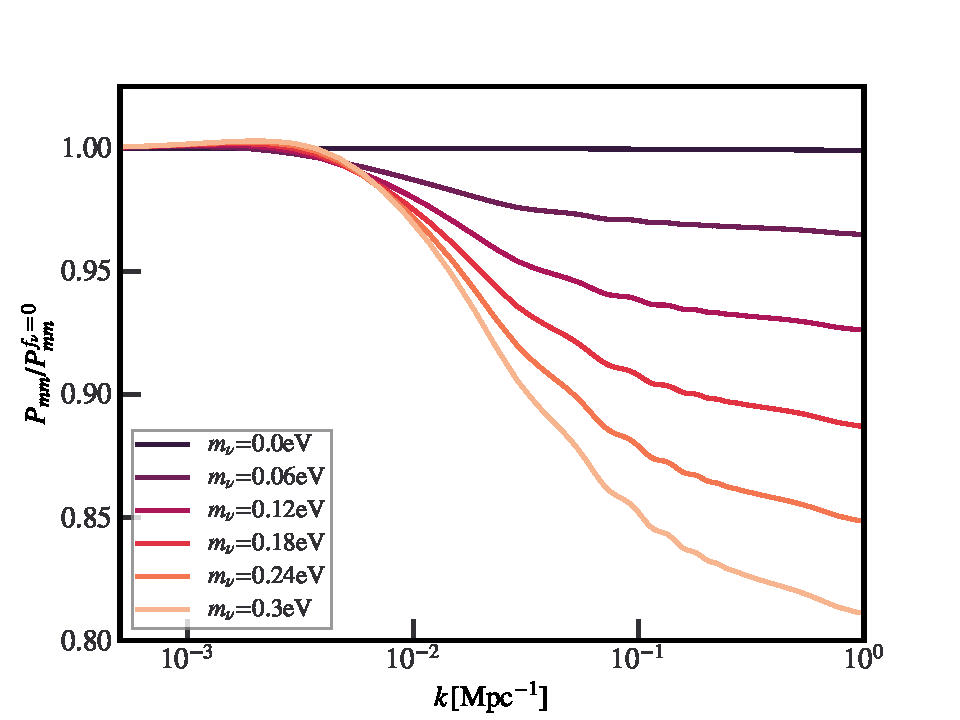
\includegraphics[width=\textwidth]{neutrinoeffect_1.pdf}
        \caption{Showing how the neutrino mass effects the matter power spectrum. For the comparasion we fixed \{$h,\Omega_b,\Omega_m$\}}
        \label{fig:mnu_suppression}
    \end{subfigure}
    \hfill
    \begin{subfigure}[b]{0.49\textwidth}
        \centering
        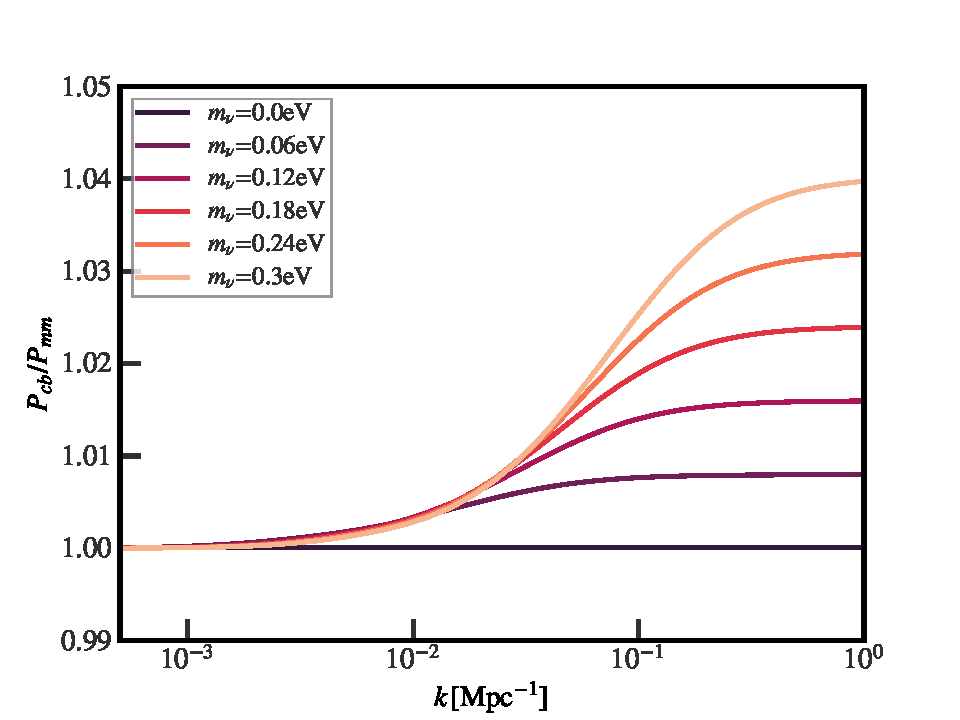
\includegraphics[width=\textwidth]{neutrinoeffect_2.pdf}
        \caption{Amplification of the CDM+baryon power spectrum for diffrent neutrino masses}
        \label{fig:PcbvPmm}  
    \end{subfigure}
       \label{fig:Mneutrino_effect} 
\end{figure}
\section{Massless Neutrinos}
The effect of additional massless neutrinos on the matter power spectrum can be spereated into backgound effects and perturbation effects. For the latter we can allready guess that these will be small. The main contribution of massless neutrinos to the matter power spectrum must happen during radiation domination as they become negligible during matter domination. During radiation domination on scales smaller than the hubble horizon it can be shown that the massless neutrinos have very little effect on the evolution of cold perturbations. This is because the massless neutrino perturbatios crossing the hubble horizon show an oscillatory behavior. When decomposing the equations of motion for the perturbations into fast ocillating modes and slowly growing modes, we see that cold matter is primaraly determend by slow modes. As a consequence we can just treat the massless neutrino perturbations as free streaming one matter domination starts.\\
The background effects of additional massive neutrinos have to be analysed a bit more carefully. Depending on what quantities are fixed other quantities need to change aswell. Firstly we start with the parametrization of additional massless relics, for this we use the parameter $N_\mathrm{eff}$. We write, that the density of total radiation is given as 
\begin{equation}
    \rho_r = \rho_\gamma\,\left[1+\frac{7}{8}\,\left(\frac{4}{11}\right)^{4/3}\,N_\mathrm{eff} \right]
\end{equation}
This means, that when fixing the densiy paramers of matter a change of $N_\mathrm{eff}$ coincides with a change of the redshift of equality, shifting the peak of the power spectrum. In order to fix the redshift of equality we need to scale $\omega_m$ as $\omega_\gamma$ is very tightly constrained by Firas.\\
The overall amplitude of the matter power spectrum is related to the amplitude of scalar perturbations $A_s$ as well as the total matter density parameter $\Omega_m$. The latter is proportional to the physical denisty of total matter by $\omega_m=\Omega_m\,h^2$. If we also want to fix the amplitude of the mater power spectrum without changeinig $A_s$ we have to scale $h$ accordingly.\\
Next if we want to substract that effect then we need to rescale the matter density. Depending on if we switch $\omega_b$ or $\omega_c$ this changes the ratio of $\omega_b/\omega_c$. This ratio is crucial in the large scale amplitude of the power spectrum as well as the amplitude of the BAOs. To cancel this effect we need to equally scale the CDM and baryon density. What would be left in this set of fixed variables is a change in $\omega_b$, that canges the phase of the BAOs. We have nolonger the freedom to fix this effect.\\
We could have also decided to fix $\omega_b$ this would need us to change the ratio of cold dark matter to baryons and suppress the large scale plateau. We illustrate the effects of changing $N_\mathrm{eff}$ for both cases in figure \ref{fig:neff_changes}. 
\begin{figure}
    \centering
    \caption{The effect of changeing Neff when fixing different quantities as explained in the Text. The Ratios where multiplied with a factor to better differentiate between them.}
    \begin{subfigure}[b]{0.49\textwidth}
        \centering
        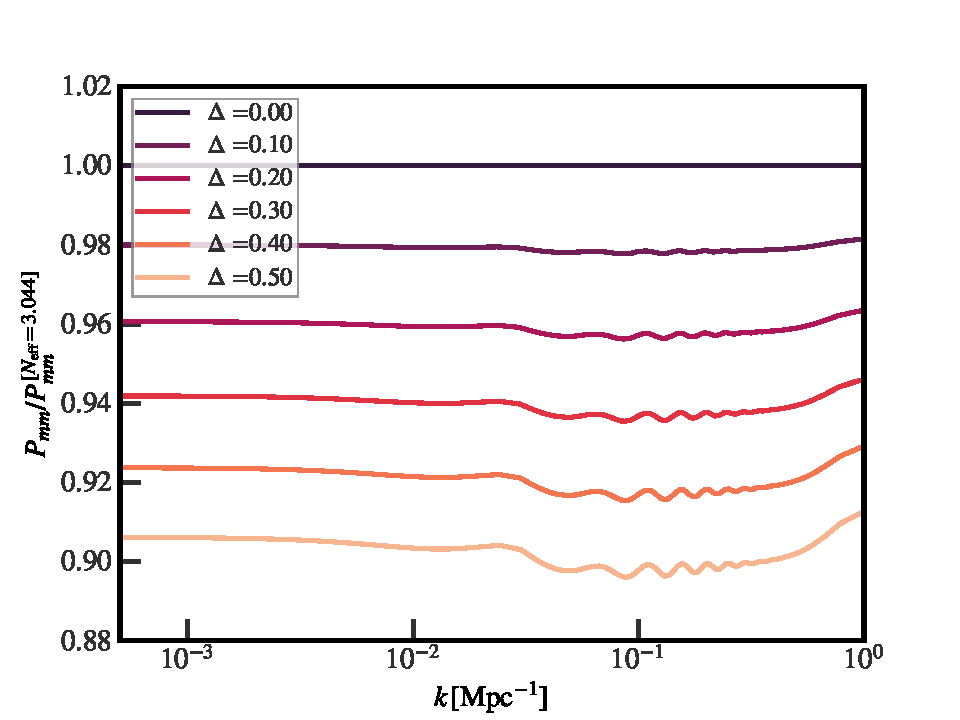
\includegraphics[width=\textwidth]{neff_luege_1.pdf}
        \caption{Fixing \{$z_\mathrm{eq},\omega_b/\omega_c,\Omega_m$\}}
        \label{fig:fixing_ratio_neff}
    \end{subfigure}
    \hfill
    \begin{subfigure}[b]{0.49\textwidth}
        \centering
        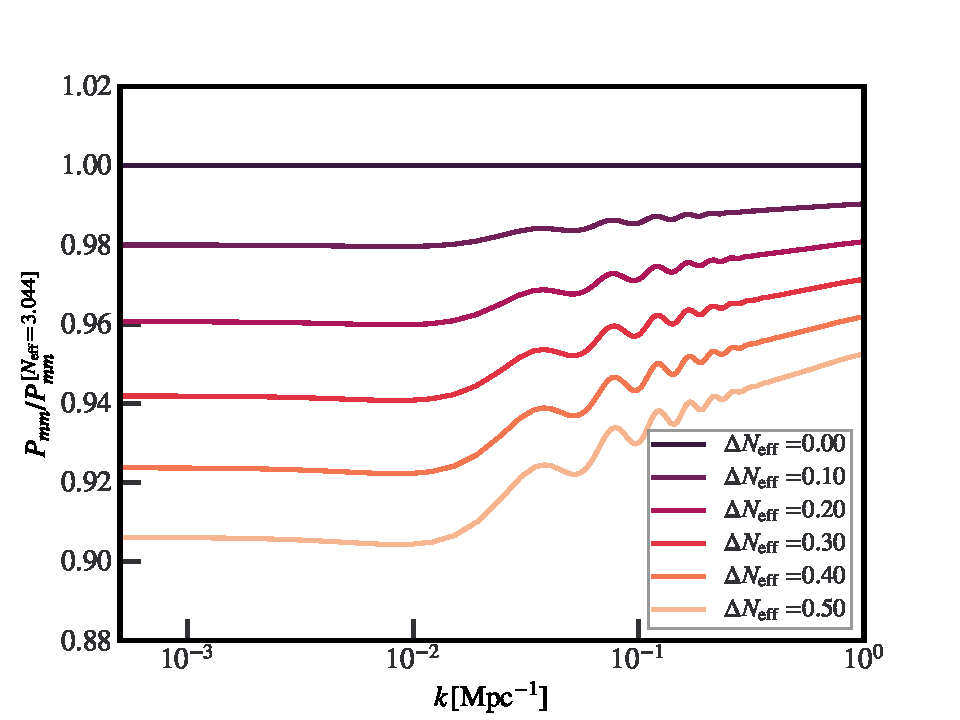
\includegraphics[width=\textwidth]{neff_luege_2.pdf}
        \caption{Fixing \{$z_\mathrm{eq},\omega_b,\Omega_m$\}}
        \label{fig:fixing_physicalb_neff}  
    \end{subfigure}
       \label{fig:neff_changes} 
\end{figure}
\end{document}